\documentclass[20pt,margin=1in,innermargin=-4.5in,blockverticalspace=-0.25in]{tikzposter}
\geometry{paperwidth=42in,paperheight=30in}
\usepackage[utf8]{inputenc}
\usepackage{amsmath}
\usepackage{amsfonts}
\usepackage{amsthm}
\usepackage{amssymb}
\usepackage{mathrsfs}
\usepackage{graphicx}
\usepackage{adjustbox}
\usepackage{enumitem}
\usepackage[backend=bibtex,style=numeric]{biblatex}
\usepackage{emory-theme}

\usepackage{mwe} % for placeholder images

\addbibresource{../reference/ref.bib}

% set theme parameters
\tikzposterlatexaffectionproofoff
\usetheme{EmoryTheme}
\usecolorstyle{EmoryStyle}

\title{Case Study : Causal Inference}
\author{Mohammed FELLAJI - Ahmed BEN AISSA \\[0.5cm]{ Supervisor : Frédéric PENNERATH \textsuperscript{$\dagger$}}}  % \textsuperscript{$\ddagger$}
\institute{\textsuperscript{$\dagger$}Associate professor at CentraleSupélec}
\titlegraphic{
\includegraphics[width=0.13\textwidth]{../figures/LogoCS.png}}

% begin document
\begin{document}
\maketitle
\centering

%%%%%%%%%%%%%%%%%%%%
\begin{columns}
%-------------------------------------
    \column{0.32}
%-------------------------------------
\block{Introduction}{
One of the most challenging questions in every problem is the one related to understanding the reason(s) why an action happened and whether or not we can explain it with the information we have at our disposal. Determining the relationships between the inputs can be done on different levels : when recording the data or even once the data collection is done. Unlike correlation, causation cannot be extracted only from the distribution of the data. Thus, the aim of this case study is analyse the different literatures on causal inference for a better understanding of this notion. \\
}
    
    
%%%%%%%%%%%%%%%%%%%%
\block{Definitions}{
Here is some of the most important definitions \cite{pearl2010mathematics, pearl2009causal} :
\begin{itemize}
\item  \textbf{Associational concept} : any relationship that can be defined in terms of a joint distribution of observed variables. For example: regression, correlation.
\item  \textbf{Causal concept} : any relationship that cannot be defined from the distribution alone. One should also rely on causal assumption that explains the different relationships. For example: randomisation, confounding.

\begin{tikzfigure}[a visualisation of the difference between causation and association]
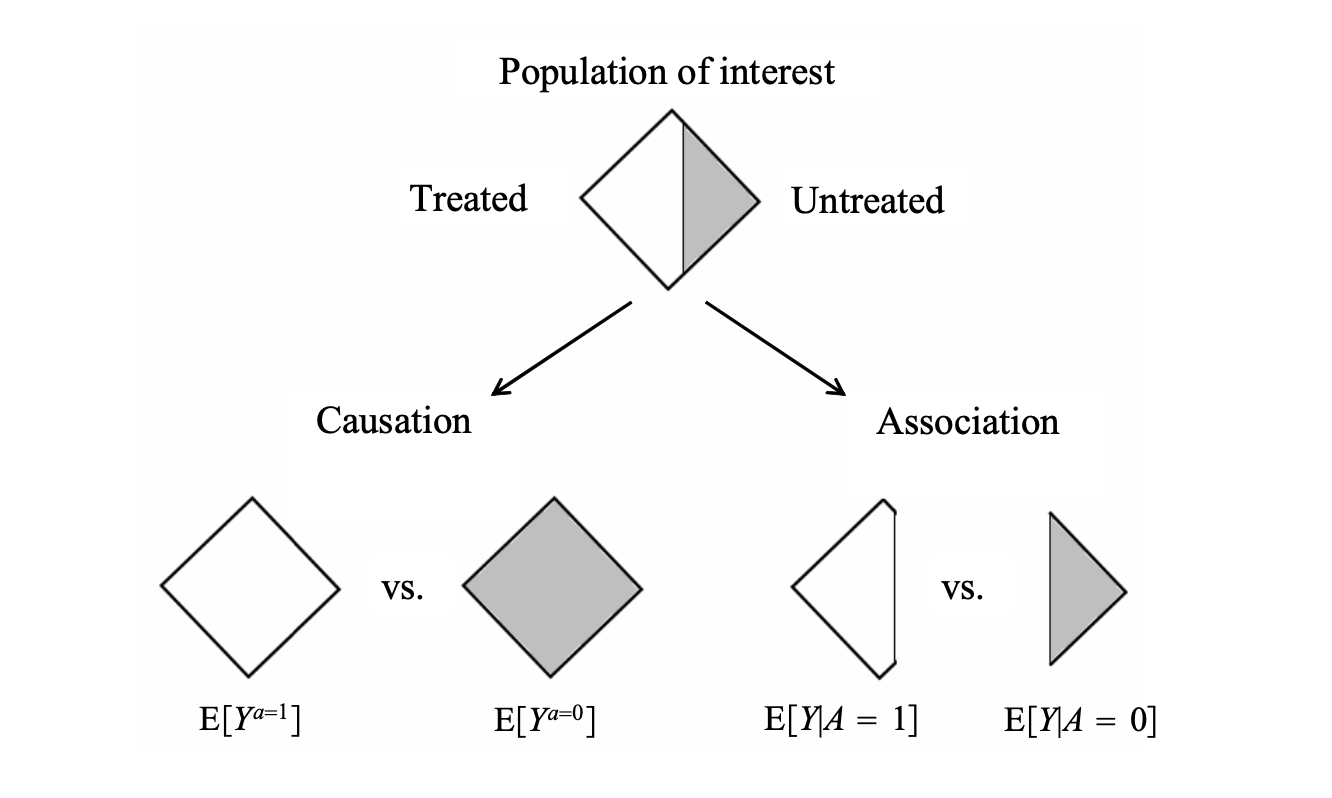
\includegraphics[width=0.7\linewidth]{../figures/asso_caus.png}
\end{tikzfigure}
        
\item \textbf{Counterfactuals} : the unobserved outcome. It is the answer to the question : what if?
\item \textbf{Confounders} : an unmeasured variable that influences both the supposed cause and the supposed effect.
\end{itemize}
}
    

%%%%%%%%%%%%%%%%%%%%
\block{Notation}{
Here is a list of some useful notations :
\begin{itemize}
\item $Y_{i}$ : random variable of the outcome for the "unit" i  (a unit is a physical object, for example, a person, at a particular point in time \cite{rubin2005causal}),
\item N : the number of units,
\item Y : ($Y_{1}$, $Y_{2}$, ..., $Y_{n}$),
\item A : treatment (a treatment is an action that can be applied or withheld from the unit \cite{rubin2005causal}),
\item $Y_{i}^{a}$ : controlled treatment 
\end{itemize}        
}

%-------------------------------------
    \column{0.36}
%-------------------------------------
%%%%%%%%%%%%%%%%%%%%
\block{Metrics and Interpretations}{
In the case of a treatment (A) that has only 2 possible values \{0,1\}, we can define these metrics: 
\begin{itemize}
\item \textbf{Individual level Causal Effect (ICE)} : the difference between an individual’s two potential outcomes.
					$$ ICE = \delta = Y_{i}^{a=1} - Y_{i}^{a=0} $$
\item \textbf{Average Causal Effect (ACE)} : it is a mesure of causation; it determines if the treatment has a causal effect on the outcome or not.
					$$ ACE = E[\delta] = E[Y^{a=1}] - E[Y^{a=0}] $$
\item \textbf{Standard estimator (S*)} : it is a mesure of association; it is computed from the treatment and control groups.  
					$$ S^{*} = E[Y^{a=1}|A=1] - E[Y^{a=0}|A=0] $$
\end{itemize}
}


%%%%%%%%%%%%%%%%%%%%
\block{Fundamental Problem of Causal Inference}{
Because one can never observe both potentiel outcomes (the outcome under different treatments), it is impossible to mesure directly the causal effects ( ACE and ICE ). This is what Holland called as the "fundamental problem of causal inference" \cite{holland1986statistics}. \\

This can be seen as missing data problem : we have $E[Y^{a=1}|A=1]$ and $E[Y^{a=0}|A=0]$ which are equal respectively to $E[Y|A=1]$ and $E[Y|A=0]$ but we don't know  $E[Y^{a=1}|A=0]$ and $E[Y^{a=1}|A=0]$. Thus, this problem can be considered as a missing data problem. 
}


\block{Randomised experimentation}{
%One of the solution to tackle the fundamental problem of causal inference is to use a randomised experience. \\

A randomised experiment is when the investigator carried out the action of interest and it was randomised because the decision to act on any study subject was made by a random device. 


\begin{tikzfigure}[an illustration of a randomised experiment]
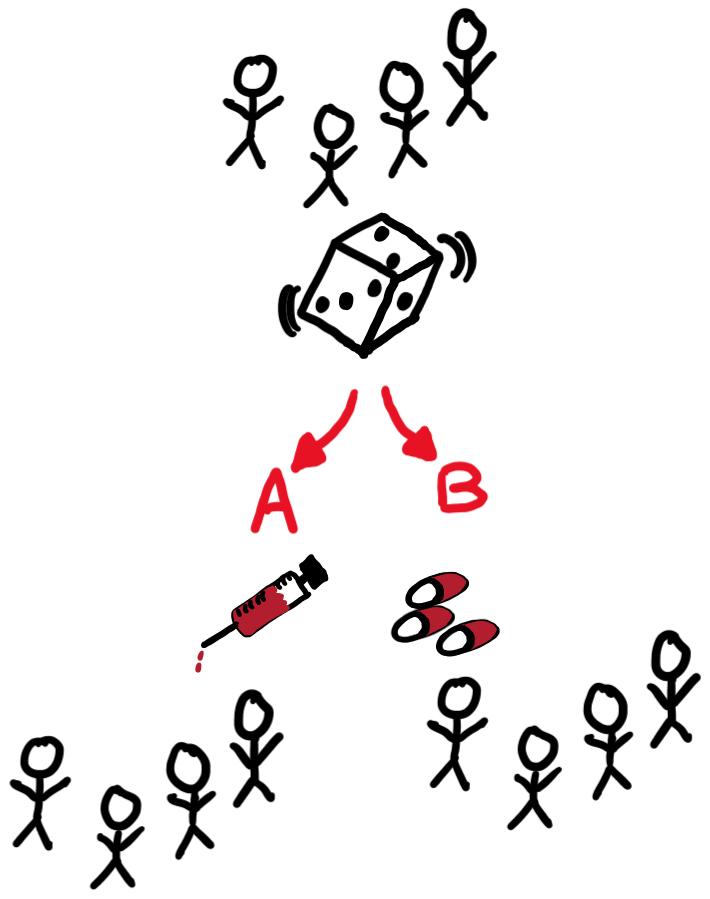
\includegraphics[width=0.3\linewidth]{../figures/random_exp.png}
\end{tikzfigure}

In the case of randomised experiment, we have the following : 

\begin{itemize}
\item $ E[Y^{a=1}|A=1] =  E[Y^{a=1}|A=0] =  E[Y^{a=1}] $   (1)
\item $ E[Y^{a=0}|A=1] =  E[Y^{a=0}|A=0] =  E[Y^{a=0}] $   (2)
\item from the equations (1) and (2) we can prove that : $ ACE = S^{*} $
\end{itemize}
}

%-------------------------------------
    \column{0.32}
%-------------------------------------
%%%%%%%%%%%%%%%%%%%%
\block{Causal discovery}{

A traditional way to discover causal relations is to use interventions or randomized experiments, which is, however, in many cases of interest too expensive, too time- consuming, unethical, or even impossible. Therefore, inferring the underlying causal structure from purely observational data, or from combinations of observational and experimental data, has drawn much attention in various disciplines. With the rapid accumulation of huge volumes of data, it is necessary to develop automatic causal search algorithms that scale well.\cite{10.3389/fgene.2019.00524}

\begin{tikzfigure}[an illustration of the PC algorithm]
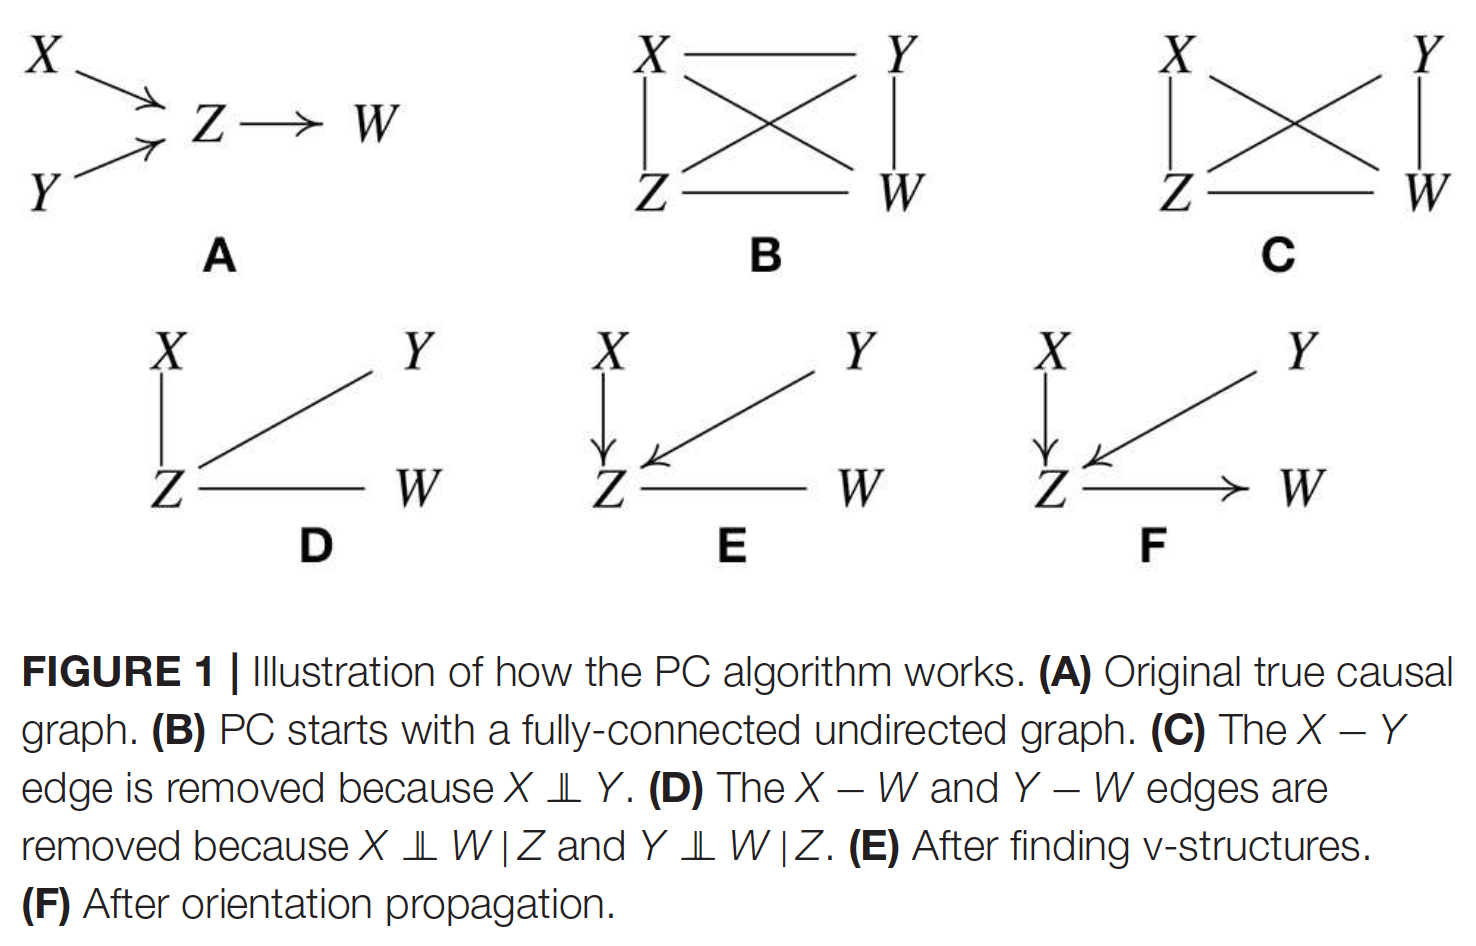
\includegraphics[width=0.5\linewidth]{../figures/PC_algorithm_1.png}
\end{tikzfigure}
}
    

%%%%%%%%%%%%%%%%%%%%
\block{Inference engine - DoWhy Library}{

\begin{tikzfigure}[The algorithm suggested by Judea Pearl \cite{pearl2019seven}]
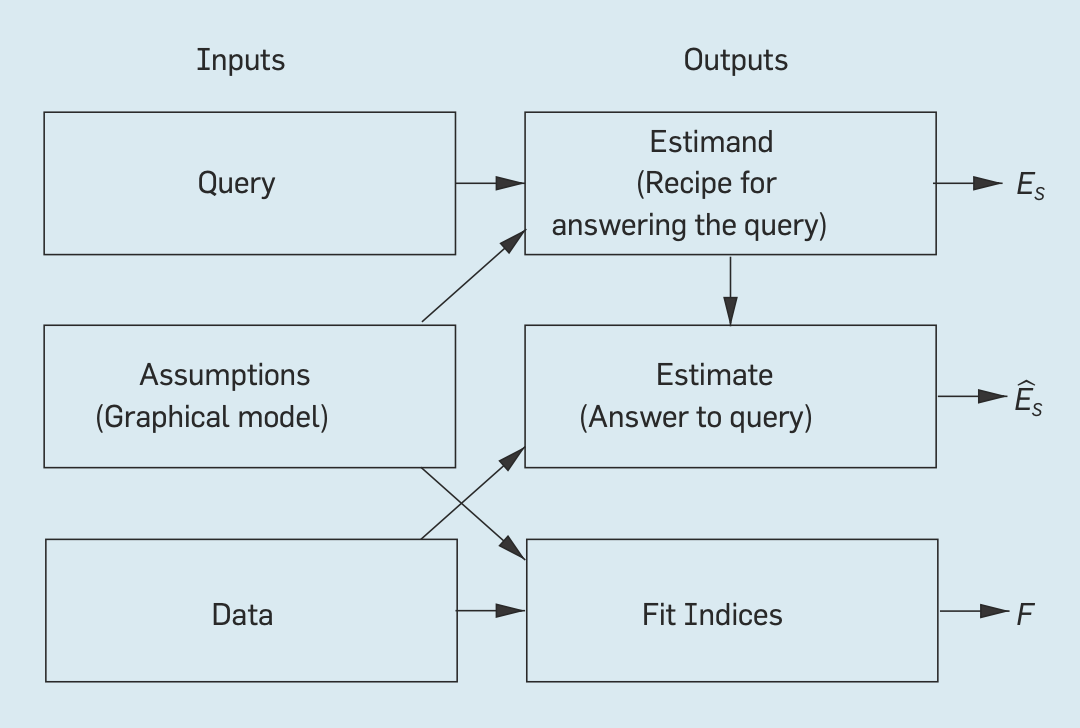
\includegraphics[width=0.5\linewidth]{../figures/inference_engine.png}
\end{tikzfigure}


}


%%%%%%%%%%%%%%%%%%%%
\block{References}{
\vspace{-1em}
\begin{footnotesize}
\printbibliography[heading=none]
\end{footnotesize}
}
    
\end{columns}
\end{document}